\part{Numerical Integrators}
\label{partNumericalMethods}

This analysis tool, which models the geometry of alveoli as a dodecahedron, requires numerical methods to integrate the constitutive equations (systems of first-order ODEs), the governing equations of motion (systems of second-order ODEs), and that integrate the length, area or volume of the finite elements (handled using Gaussian quadrature).  The numerical methods used in this work are discussed below.

\section{ODE Solvers}

The various constitutive equations that describe our alveolar model present themselves as ordinary differential equations that need to be integrated.  To this end, we employ the PECE (Predict, Evaluate, Correct, re-Evaluate) algorithms of Freed \cite{Freed17a} which are suitable for solving stiff systems of first- and second-order, ordinary, differential equations.  These methods are based upon Gear's well-known second-order backward difference formula (BDF2, which is Eqn.~\ref{1stOrderCorrector} below).

Time $t$ is considered to be the independent variable, discretized over an interval in time $[t_0, t_N]$ for which $N$ solutions are to be extracted at nodes $n=1, 2, \ldots, N$ spaced at uniform intervals in time with a common step size of $h = (t_N - t_0)/N$ separating them, where time $t_0$ associates with the initial conditions.  This is the \textit{global step size\/} at which solutions are to be gathered.  A dynamically controlled \textit{local step size}, whose size is adjusted on the fly to manage truncation error, is implemented into the code according to a scheme put forward in Ref.~\cite{Soderlind02}.  Solver interfaces are listed in \ref{appSolvers}.

\subsection{PECE Solver for First-Order ODEs}
\label{sec:1stOrderPECE}

Let $\mathbf{x}$ be a vector of dependent variables obeying a differential equation of evolution $\mathrm{d} \mathbf{x}(t) / \mathrm{d} t = \dot{\mathbf{x}} = \mathbf{f} (t, \mathbf{x})$ subject to an initial condition $\mathbf{x}_0 = \mathbf{x}(t_0)$ where $t$ is the independent variable, typically time, but not in our case.

The two-step method put forward here incrementally solves such an ODE, returning solutions associated with the next moment in time $t_{n+1}$, i.e., it acquires $\mathbf{x}_{n+1}$, given knowledge of the  previous $\mathbf{x}_{n-1}$ and current $\mathbf{x}_n$ solutions plus their rates $\dot{\mathbf{x}}_{n-1}$ and $\dot{\mathbf{x}}_n$ with the corrector also depending upon $\dot{\mathbf{x}}_{n+1}$, i.e., the corrector is an implicit method.

\subsubsection{Start-Up Algorithm}

Multi-step methods are not self starting; consequently, Heun's method (a forward-Euler predictor with a trapezoidal corrector) is used here to start our integrator; specifically,
\begin{subequations}
    \label{startUp1stOrderODEs}
    \begin{align}
    \mbox{} & \text{Predict} & 
    \mathbf{x}_1^p & = \mathbf{x}_0 + h \dot{\mathbf{x}}_0 + \mathcal{O} (h^2)
    \label{startUp1stOrderPredictor} \\
    \mbox{} & \text{Evaluate} & 
    \dot{\mathbf{x}}^p_1 & = \mathbf{f} (t_1 , \mathbf{x}_1^p) 
    \label{startUp1stEvaluate} \\
    \mbox{} & \text{Correct} &
    \mathbf{x}_1 & = \mathbf{x}_0 + \tfrac{1}{2} h 
    \bigl( \dot{\mathbf{x}}_1^p + \dot{\mathbf{x}}_0 \bigr) + \mathcal{O} (h^3)
    \label{startUp1stOrderCorrector} \\
    \mbox{} & \text{Re-Evaluate} & 
    \dot{\mathbf{x}}_1 & = \mathbf{f} (t_1 , \mathbf{x}_1) 
    \label{startUp1stReEvaluate}
    \end{align}
\end{subequations}
wherein $\dot{\mathbf{x}}_0 = \mathbf{f}(t_0, \mathbf{x}_0)$ and $t_1 = t_0 + h$.  The correct\slash re-evaluate steps can be iterated over until a convergence criterion is satisfied, if need be.

\subsubsection{Two-Step ODE Solver}

The two-step method of Freed \cite{Freed17a} for solving $1^{\text{st}}$ order ODEs is
\begin{subequations}
    \label{1stOrderODEs}
    \begin{align}
    \mbox{} & \text{Predict} & 
    \mathbf{x}_{n+1}^p & = \tfrac{1}{3} 
    \bigl( 4 \mathbf{x}_n - \mathbf{x}_{n-1} \bigr) + 
    \tfrac{2}{3} h \bigl( 2 \dot{\mathbf{x}}_n - \dot{\mathbf{x}}_{n-1} 
    \bigr) + \mathcal{O} (h^3)
    \label{1stOrderPredictor} \\
    \mbox{} & \text{Evaluate} & 
    \dot{\mathbf{x}}^p_{n+1} & = \mathbf{f} (t_{n+1} , \mathbf{x}_{n+1}^p) 
    \label{1stOrderEvaluate} \\
    \mbox{} & \text{Correct} &
    \mathbf{x}_{n+1} & = \tfrac{1}{3} 
    \bigl( 4 \mathbf{x}_n - \mathbf{x}_{n-1} \bigr) + 
    \tfrac{2}{3} h \dot{\mathbf{x}}^{p}_{n+1} + \mathcal{O} (h^3)
    \label{1stOrderCorrector} \\
    \mbox{} & \text{Re-Evaluate} & 
    \dot{\mathbf{x}}_{n+1} & = \mathbf{f} (t_{n+1} , \mathbf{x}_{n+1}) 
    \label{1stOrderReEvaluate}
    \end{align}
\end{subequations} 
where $t_{n+1} = t_n + h$.  This corrector is the well-known BDF2 formula of Gear to which Freed provided a predictor.  The correct\slash re-evaluate steps can be iterated over until a convergence criterion is satisfied, if need be.  Implementation of this integrator is found in \ref{app1stOrderODEs}.  

For both the predictor and corrector, solution $\mathbf{x}$ has a weight of 1, while its rate $\dot{\mathbf{x}}$ has a weight of $\tfrac{2}{3} h$; hence, this predictor\slash corrector pair is consistent.

\subsection{A Relevant Example}

In our finite element implementation, a hypo-elastic material model \cite{Truesdell55} is introduced to describe the constitutive response of an alveolus in that
\begin{displaymath}
    \dot{\boldsymbol{\sigma}} = \mathbf{M} ( \boldsymbol{\sigma} , \boldsymbol{\epsilon} ) \, \dot{\boldsymbol{\epsilon}} 
    \quad \text{or equivalently \cite{Noll55}} \quad
    \mathrm{d} \boldsymbol{\sigma} = \mathbf{M} ( \boldsymbol{\sigma} , \boldsymbol{\epsilon} ) \, \mathrm{d} \boldsymbol{\epsilon}
\end{displaymath} 
where $\boldsymbol{\epsilon}$ is a vector of thermo\-dynamic strains, $\boldsymbol{\sigma}$ is a vector of thermo\-dynamic stresses, and $\mathbf{M}$ is a square matrix comprised of their tangent moduli, which can depend both upon stress and strain.  In our application, the thermo\-dynamic stress attributes are 
\begin{displaymath}
   \boldsymbol{\sigma}_{1D} = \{ \eta , s \} , \quad
   \boldsymbol{\sigma}_{2D} = \{ \eta , s^{\pi} , s^{\sigma} , s^{\tau} \}^{\mathsf{T}} , \quad
   \boldsymbol{\sigma}_{3D} = \{ \eta , \Pi , \sigma_1 , \sigma_2 , \tau_1 , \tau_2 , \tau_3 \}^{\mathsf{T}}
\end{displaymath}
where $\eta$ is entropy and the rest are stresses, whose thermo\-dynamic conjugates are the strain attributes
\begin{displaymath}
\boldsymbol{\epsilon}_{1D} = \{ \theta , e \} , \quad
\boldsymbol{\epsilon}_{2D} = \{ \theta , \xi , \varepsilon , \gamma \}^{\mathsf{T}} , \quad
\boldsymbol{\epsilon}_{3D} = \{ \theta , \Xi , \varepsilon_1 , \varepsilon_2 , \gamma_1 , \gamma_2 , \gamma_3 \}^{\mathsf{T}}
\end{displaymath}
where $\theta$ is temperature and the rest are strains.  In the 2- and 3-D cases, these stress-strain attributes arise from Gram-Schmidt decompositions of the deformation gradient (cf.\ \S\ref{secQR2D}, \S\ref{secConjugatePairs} and \S\ref{secFE_CE}).  Constructing tangent moduli $\mathbf{M} ( \boldsymbol{\sigma} , \boldsymbol{\epsilon} )$ is the topic of Part~\ref{partConstitutive}.  In the above problem, the thermo\-dynamic strains $\boldsymbol{\epsilon}$ and their differential rates $\mathrm{d} \boldsymbol{\epsilon}$ are known, it is their stresses $\boldsymbol{\sigma}$ that must be integrated.  Both $\boldsymbol{\sigma}$ and $\mathrm{d} \boldsymbol{\sigma} = \mathbf{M} \, \mathrm{d} \boldsymbol{\epsilon}$ arise in the construction of our stiffness matrices, cf.\ \S\ref{secStiffnessMatrices}.

Equation (\ref{startUp1stOrderODEs}) is used to take the first step of integration; specifcally, 
\begin{subequations}
    \notag
    \begin{align}
    \mbox{} & \text{Predict} & 
    \boldsymbol{\sigma}_1^p & = \boldsymbol{\sigma}_0 + h \, \mathrm{d} \boldsymbol{\sigma}_0 \\
    \mbox{} & \text{Evaluate} & 
    \mathrm{d} \boldsymbol{\sigma}^p_1 & = \mathbf{M} ( \boldsymbol{\sigma}_1^p ,
    \boldsymbol{\epsilon} ) \, \mathrm{d} \boldsymbol{\epsilon}_1 \\
    \mbox{} & \text{Correct} &
    \boldsymbol{\sigma}_1 & = \boldsymbol{\sigma}_0 + \tfrac{1}{2} h 
    \bigl( \mathrm{d} \boldsymbol{\sigma}_1^p + 
    \mathrm{d} \boldsymbol{\sigma}_0 \bigr) \\
    \mbox{} & \text{Re-Evaluate} & 
    \mathrm{d} \boldsymbol{\sigma}_1 & = \mathbf{M} ( \boldsymbol{\sigma}_1 , 
    \boldsymbol{\epsilon}_1) \, \mathrm{d} \boldsymbol{\epsilon}_1
    \end{align}
\end{subequations}
where $\mathrm{d} \boldsymbol{\sigma}_0 = \mathbf{M} ( \boldsymbol{\sigma}_0 , \boldsymbol{\epsilon}_0) \, \mathrm{d} \boldsymbol{\epsilon}_0$, with the remaining steps of integration following according to Eqn.~(\ref{1stOrderODEs}), specifically
\begin{subequations}
    \notag
    \begin{align}
    \mbox{} & \text{Predict} & 
    \boldsymbol{\sigma}_{n+1}^p & = \tfrac{1}{3} 
    \bigl( 4 \boldsymbol{\sigma}_n - \boldsymbol{\sigma}_{n-1} \bigr) + 
    \tfrac{2}{3} h \bigl( 2 \, \mathrm{d} \boldsymbol{\sigma}_n - 
    \mathrm{d} \boldsymbol{\sigma}_{n-1} \bigr) \\
    \mbox{} & \text{Evaluate} & 
    \mathrm{d} \boldsymbol{\sigma}^p_{n+1} & = \mathbf{M} ( \boldsymbol{\sigma}_{n+1}^p , \boldsymbol{\epsilon}_{n+1} ) \, 
    \mathrm{d} \boldsymbol{\epsilon}_{n+1} \\
    \mbox{} & \text{Correct} &
    \boldsymbol{\sigma}_{n+1} & = \tfrac{1}{3} 
    \bigl( 4 \boldsymbol{\sigma}_n - \boldsymbol{\sigma}_{n-1} \bigr) + 
    \tfrac{2}{3} h \, \mathrm{d} \boldsymbol{\sigma}^{p}_{n+1}  \\
    \mbox{} & \text{Re-Evaluate} & 
    \mathrm{d} \boldsymbol{\sigma}_{n+1} & = \mathbf{M} ( 
    \boldsymbol{\sigma}_{n+1} , \boldsymbol{\epsilon}_{n+1} )  \,
    \mathrm{d} \boldsymbol{\epsilon}_{n+1}
    \end{align}
\end{subequations} 
where the differential strain rates $\mathrm{d} \boldsymbol{\epsilon}$ are computed via finite differences according to \S\ref{secFE_CE}.


\subsection{PECE Solver for Second-Order ODEs}
\label{sec:2ndOrderPECE}

Let $\mathbf{x}$ be a vector of dependent variables obeying a differential equation of evolution $\mathrm{d}^2 \mathbf{x}(t) / \mathrm{d} t^2 = \ddot{\mathbf{x}} = \mathbf{f} (t, \mathbf{x}, \dot{\mathbf{x}})$ subject to initial conditions $\mathbf{x}_0 = \mathbf{x}(t_0)$ and $\dot{\mathbf{x}}_0 = \dot{\mathbf{x}}(t_0)$.  One may think of $\mathbf{x}$ as being displacements and their rates $\mathbf{v} = \dot{\mathbf{x}}$ as being velocities with $\mathbf{a} = \dot{\mathbf{v}} = \ddot{\mathbf{x}}$ representing accelerations. 

The two-step method put forward here incrementally solves such an ODE, returning solutions associated with the next moment in time $t_{n+1}$, i.e., it acquires $\mathbf{x}_{n+1}$ \& $\dot{\mathbf{x}}_{n+1}$ given knowledge of the previous $\mathbf{x}_{n-1}$ \& $\dot{\mathbf{x}}_{n-1}$ and current $\mathbf{x}_n$ \& $\dot{\mathbf{x}}_n$ solutions plus their accelerations $\ddot{\mathbf{x}}_{n-1}$ and $\ddot{\mathbf{x}}_n$ with the corrector also depending upon $\ddot{\mathbf{x}}_{n+1}$, i.e., the corrector is an implicit method.

\subsubsection{Start-Up Algorithm}

Multi-step methods are not self starting, so a one-step method is needed to take the first step of integration, specifically
\begin{subequations}
    \label{pairedStartUp}
    \begin{align}
    \mbox{} & \text{Predict} & 
    \mathbf{x}_1^p & = \mathbf{x}_0 + h \dot{\mathbf{x}}_0 +
    \tfrac{1}{2} h^2 \ddot{\mathbf{x}}_0 + \mathcal{O} (h^3) 
    \label{startupDisplacementPredictor} \\
    \mbox{} & &
    \dot{\mathbf{x}}^p_1 & = \dot{\mathbf{x}}_0 + h \ddot{\mathbf{x}}_0 + 
    \mathcal{O} (h^2) 
    \label{startUpVelocityPredictor} \\
    \mbox{} & \text{Evaluate} &
    \ddot{\mathbf{x}}^p_1 & = \mathbf{f} (t_1, \mathbf{x}^p_1, \dot{\mathbf{x}}^p_1)
    \label{startUpEvaluate} \\
    \mbox{} & \text{Correct} &
    \mathbf{x}_1 & = \mathbf{x}_0 + \tfrac{1}{2} h 
    \bigl( \dot{\mathbf{x}}^p_1 + \dot{\mathbf{x}}_0 \bigr) -
    \tfrac{1}{12} h^2 \bigl( \ddot{\mathbf{x}}^p_1 - 
    \ddot{\mathbf{x}}_0 \bigr) + \mathcal{O} (h^4) 
    \label{startupDisplacementCorrector} \\
    \mbox{} & &
    \dot{\mathbf{x}}_1 & = \dot{\mathbf{x}}_0 + \tfrac{1}{2} h 
    \bigl( \ddot{\mathbf{x}}_1^p + \ddot{\mathbf{x}}_0 \bigr) + 
    \mathcal{O} (h^3)
    \label{startUpVelocityCorrector} \\
    \mbox{} & \text{Re-Evaluate} &
    \ddot{\mathbf{x}}_1 & = \mathbf{f} (t_1, \mathbf{x}_1, \dot{\mathbf{x}}_1) 
    \label{startUpReEvaluate}
    \end{align}
\end{subequations}
wherein $\ddot{\mathbf{x}}_0 = \mathbf{f}(t_0, \mathbf{x}_0, \dot{\mathbf{x}}_0)$ and $t_1 = t_0 + h$.  The correct\slash re-evaluate steps can be iterated over until a convergence criterion is satisfied, if need be.

\subsubsection{Two-Step ODE Solver}

The two-step method of Freed \cite{Freed17a} for solving $2^{\text{nd}}$ order ODEs is
\begin{subequations}
    \label{pairedMethods}
    \begin{align}
    \mbox{} & \text{Predict} &
    \mathbf{x}_{n+1}^p & = \tfrac{1}{3} \bigl(
    4 \mathbf{x}_n - \mathbf{x}_{n-1} \bigr) + 
    \tfrac{1}{6} h \bigl( 3 \dot{\mathbf{x}}_n + 
    \dot{\mathbf{x}}_{n-1} \bigr) \notag \\ 
    \mbox{} & & & \hspace{3.175cm} + 
    \tfrac{1}{36} h^2 \bigl( 31 \ddot{\mathbf{x}}_n - 
    \ddot{\mathbf{x}}_{n-1} \bigr) + \mathcal{O} (h^4) 
    \label{displacementPredictor} \\
    \mbox{} & &
    \dot{\mathbf{x}}_{n+1}^p & = \tfrac{1}{3} 
    \bigl( 4 \dot{\mathbf{x}}_n - \dot{\mathbf{x}}_{n-1} \bigr) + 
    \tfrac{2}{3} h \bigl( 2\ddot{\mathbf{x}}_n - \ddot{\mathbf{x}}_{n-1} 
    \bigr) + \mathcal{O} (h^3)
    \label{velocityPredictor} \\
    \mbox{} & \text{Evaluate} &
    \ddot{\mathbf{x}}^p_{n+1} & = \mathbf{f} (t_{n+1}, \mathbf{x}^p_{n+1}, \dot{\mathbf{x}}^p_{n+1}) 
    \label{2ndEvaluate} \\
    \mbox{} & \text{Correct} & 
    \mathbf{x}_{n+1} & = \tfrac{1}{3} \bigl(
    4  \mathbf{x}_n - \mathbf{x}_{n-1} \bigr) +
    \tfrac{1}{24} h \bigl( \dot{\mathbf{x}}^p_{n+1} +
    14 \dot{\mathbf{x}}_n + \dot{\mathbf{x}}_{n-1} \bigr) 
    \notag \\
    \mbox{} & & & \hspace{3.175cm} +
    \tfrac{1}{72} h^2 \bigl( 10 \ddot{\mathbf{x}}^p_{n+1} + 
    51 \ddot{\mathbf{x}}_n - \ddot{\mathbf{x}}_{n-1} \bigr) + 
    \mathcal{O} (h^4)
    \label{displacementCorrector} \\ 
    \mbox{} & &
    \dot{\mathbf{x}}_{n+1} & = \tfrac{1}{3} 
    \bigl( 4 \dot{\mathbf{x}}_n - \dot{\mathbf{x}}_{n-1} \bigr) + 
    \tfrac{2}{3} h \ddot{\mathbf{x}}^p_{n+1} + \mathcal{O} (h^3)
    \label{velocityCorrector} \\
    \mbox{} & \text{Re-Evaluate} & 
    \ddot{\mathbf{x}}_{n+1} & = \mathbf{f} (t_{n+1}, \mathbf{x}_{n+1}, \dot{\mathbf{x}}_{n+1})
    \label{2ndReEvaluate}
    \end{align}
\end{subequations}
where $t_{n+1} = t_n + h$.  An implementation of this integrator is described in \ref{app2ndOrderODEs}.  

The above PECE solver for velocity $\dot{\mathbf{x}}$ is the same method presented in Eq.~(\ref{1stOrderODEs}), so this predictor\slash corrector pair is consistent.  Likewise, in both the predictor and corrector for displacement $\mathbf{x}$, contributions from the solution $\mathbf{x}$ have a weight of 1, contributions from the velocities $\dot{\mathbf{x}}$ have a weight of $\tfrac{2}{3} h$, and contributions from the accelerations $\ddot{\mathbf{x}}$ have a weight of $\tfrac{5}{6} h^2$; hence, this predictor\slash corrector pair is consistent, too.

\subsection{A Relevant Example}
\label{sec:solve2ndOrderODE}

The finite element problem that we consider here requires solutions for
\begin{displaymath}
    \mathbf{M} \ddot{\mathbf{u}} + \mathbf{K}\mathbf{u} = \mathbf{f}(t)
\end{displaymath}
where $\mathbf{u}$ is a generalized displacement vector, $\ddot{\mathbf{u}}$ is its acceleration, $\mathbf{M}$ and $\mathbf{K}$ are mass and stiffness matrices, and $\mathbf{f}(t)$ is a forcing function evaluated at current time $t$.  For this system of ODEs, the first step to be taken follows algorithm (\ref{pairedStartUp}) and is implemented as
\begin{subequations}
    \notag
    \begin{align}
    \mbox{} & \text{Predict} & 
    \mathbf{u}_1^p & = \mathbf{u}_0 + h \dot{\mathbf{u}}_0 +
    \tfrac{1}{2} h^2 \ddot{\mathbf{u}}_0 \\
    \mbox{} & &
    \dot{\mathbf{u}}^p_1 & = \dot{\mathbf{u}}_0 + h \ddot{\mathbf{u}}_0 \\
    \mbox{} & \text{Evaluate} &
    \ddot{\mathbf{u}}^p_1 & = \mathbf{M}^{-1} \bigl( \mathbf{f}(t_{1} ) - 
    \mathbf{K} \mathbf{u}_1^p \bigr) \\
    \mbox{} & \text{Correct} &
    \mathbf{u}_1 & = \mathbf{u}_0 + \tfrac{1}{2} h 
    \bigl( \dot{\mathbf{u}}^p_1 + \dot{\mathbf{u}}_0 \bigr) -
    \tfrac{1}{12} h^2 \bigl( \ddot{\mathbf{u}}^p_1 - \ddot{\mathbf{u}}_0 \bigr) \\
    \mbox{} & &
    \dot{\mathbf{u}}_1 & = \dot{\mathbf{u}}_0 + \tfrac{1}{2} h 
    \bigl( \ddot{\mathbf{u}}_1^p + \ddot{\mathbf{u}}_0 \bigr) \\
    \mbox{} & \text{Re-Evaluate} &
    \ddot{\mathbf{u}}_1 & = \mathbf{M}^{-1} \bigl( \mathbf{f}(t_1 ) - 
    \mathbf{K} \mathbf{u}_1 \bigr)
    \end{align}
\end{subequations}
where the CE steps of the PECE sequence can be iterated on to a user-specified tolerance, which increases the methods stability as the corrector is implicit.  Continued solution steps are then governed by algorithm (\ref{pairedMethods}), which takes on the form of
\begin{subequations}
    \notag
    \begin{align}
    \mbox{} & \text{Predict} &
    \mathbf{u}_{n+1}^p & = \tfrac{1}{3} \bigl(
    4 \mathbf{u}_n - \mathbf{u}_{n-1} \bigr) + 
    \tfrac{1}{6} h \bigl( 3 \dot{\mathbf{u}}_n + 
    \dot{\mathbf{u}}_{n-1} \bigr) + 
    \tfrac{1}{36} h^2 \bigl( 31 \ddot{\mathbf{u}}_n - 
    \ddot{\mathbf{u}}_{n-1} \bigr) \\
    \mbox{} & &
    \dot{\mathbf{u}}_{n+1}^p & = \tfrac{1}{3} 
    \bigl( 4 \dot{\mathbf{u}}_n - \dot{\mathbf{u}}_{n-1} \bigr) + 
    \tfrac{2}{3} h \bigl( 2 \ddot{\mathbf{u}}_n - \ddot{\mathbf{u}}_{n-1} \bigr) \\
    \mbox{} & \text{Evaluate} &
    \ddot{\mathbf{u}}^p_{n+1} & = \mathbf{M}^{-1} \bigl( \mathbf{f}(t_{n+1} ) - 
    \mathbf{K} \mathbf{u}_{n+1}^p \bigr) \\
    \mbox{} & \text{Correct} & 
    \mathbf{u}_{n+1} & = \tfrac{1}{3} \bigl(
    4  \mathbf{u}_n - \mathbf{u}_{n-1} \bigr) +
    \tfrac{1}{24} h \bigl( \dot{\mathbf{u}}^p_{n+1} +
    14 \dot{\mathbf{u}}_n + \dot{\mathbf{u}}_{n-1} \bigr)  \\
    \mbox{} & & & \hspace{3.175cm} +
    \tfrac{1}{72} h^2 \bigl( 10 \ddot{\mathbf{u}}^p_{n+1} + 
    51 \ddot{\mathbf{u}}_n - \ddot{\mathbf{u}}_{n-1} \bigr) \\ 
    \mbox{} & &
    \dot{\mathbf{u}}_{n+1} & = \tfrac{1}{3} 
    \bigl( 4 \dot{\mathbf{u}}_n - \dot{\mathbf{u}}_{n-1} \bigr) + 
    \tfrac{2}{3} h \ddot{\mathbf{u}}^p_{n+1}  \\
    \mbox{} & \text{Re-Evaluate} & 
    \ddot{\mathbf{u}}_{n+1} & = \mathbf{M}^{-1} \bigl( \mathbf{f}(t_{n+1} ) - 
    \mathbf{K} \mathbf{u}_{n+1} \bigr) 
    \end{align}
\end{subequations}
where, again, the CE steps of the PECE sequence can be iterated on to a user-specified tolerance.  In this problem, velocities $\dot{\mathbf{u}}$ are not needed for the evaluation steps, but they are required by the prediction and correction steps of integration.

We observe that the mass matrix must not be ill conditioned in order for this algorithm to work as intended.  Since the mass matrix does not change with time, it only needs to be evaluated and inverted once.  This is an advantage over using the popular Newmark \cite{Newmark59} integrator where matrix inversion is required at every step along a solution path.

\section{Quadrature Rules for Spatial Integration}
\label{secGauss}

Three Gauss quadrature rules are given here for alveolar chords, alveolar septa and for tetrahedra that fill an alveolar sac.  These formul\ae\ integrate polynomials of $1^{\text{st}}$, $3^{\text{rd}}$ and $5^{\text{th}}$ degrees, exactly, for the chord and pentagon, and of $1^{\text{st}}$, $2^{\text{nd}}$ and $3^{\text{rd}}$ degrees, exactly, for a tetrahedron.  In all cases, integrating $1^{\text{st}}$ order polynomials takes place at their centroids.

\subsection{Gauss Integration of Alveolar Chords}

The quadrature rules that integrate a 1D chord in its natural co-ordinate system, which spans $-1 \leq \xi \leq 1$, are presented in Table~\ref{tabQuadrature1D}.  These formul\ae\ are well known and can be found in most finite element textbooks.

\begin{table}
    \centering
    \begin{tabular}{|c|rr|}
        \hline
        node & \centering $\xi$ co-ordinate \phantom{1}  & 
        weight \phantom{123} \\ \hline
        & \multicolumn{2}{|c|}{Exact for Polynomials of Degree $1^{\phantom{|^|}}$} \\ 
        \hline
        1 & 0.000000000000 & 2.000000000000 \\ 
        \hline
        & \multicolumn{2}{|c|}{Exact for Polynomials of Degree $3^{\phantom{|^|}}$} \\ \hline
        1 & -0.577350269189 & 1.000000000000\\
        2 & 0.577350269189 & 1.000000000000\\ 
        \hline
        & \multicolumn{2}{|c|}{Exact for Polynomials of Degree $5^{\phantom{|^|}}$} \\ \hline
        1 & -0.774596669241 & 0.555555555556 \\
        2 & 0.000000000000 & 0.888888888889\\
        3 & 0.774596669241 & 0.555555555556\\ 
        \hline
    \end{tabular}
    \caption{Generalized, Gaussian, quadrature weights and nodes for integrating over an alveolar chord in its natural co-ordinate system.  These weights sum to 2, the span of its natural co-ordinate.  We note that $1/\sqrt{3} \approx 0.577350269189$ and that $\sqrt{3/5} \approx 0.774596669241$.}
    \label{tabQuadrature1D}
\end{table}

\subsection{Gauss Integration of Alveolar Septa}

Three, Gauss, quadrature rules for a regular pentagon described in its natural coordinate system, i.e., oriented according to Fig.~\ref{figRegPentagon}, are presented in Table~\ref{tabQuadrature}.  These quadratures exactly integrate polynomials of order 1, 3 and 5, respectively.  They were supplied to the authors by Prof.\ N.\ Sukumar from the University of California at Davis, which he derived for us at our request using a methodology that he published in \cite{Mousavietal10}.  In that document, the authors derived formul\ae\ for determining the nodes and weights for a class of generalized, Gaussian, quadrature rules, which they then applied to pentagons, hexagons, heptagons and octagons, of which they only published their nodes and weights of quadrature for the hexagon, as it tiles two space.  The node for the $1^{\mathrm{st}}$ order method is located at the centroid.  Nodes for the $3^{\mathrm{rd}}$ and $5^{\mathrm{th}}$ order methods of Table~\ref{tabQuadrature} are displayed in Fig.~\ref{figQuadrature}.

\begin{table}
    \centering
    \begin{tabular}{|c|rrr|}
        \hline
        node & \centering $\xi$ coordinate \phantom{123}  & 
        $\eta$ coordinate \phantom{123} & weight \phantom{12345} \\ \hline
        & \multicolumn{3}{|c|}{Exact for Polynomials of Degree $1^{\phantom{|^|}}$} \\ \hline
        1 & 0.0000000000000000 & 0.0000000000000000 &
        2.3776412907378837\vphantom{$|^{|^|}$} \\ 
        \hline
        & \multicolumn{3}{|c|}{Exact for Polynomials of Degree $3^{\phantom{|^|}}$} \\ \hline
        1 & -0.0349156305831802 &  0.6469731019095136 &
        0.5449124407446143\vphantom{$|^{|^|}$} \\
        2 & -0.5951653065516678 & -0.0321196846022659 & 0.6439082046243272 \\
        3 &  0.0349156305831798 & -0.6469731019095134 & 0.5449124407446146 \\
        4 &  0.5951653065516677 &  0.0321196846022661 & 0.6439082046243275 \\ 
        \hline
        & \multicolumn{3}{|c|}{Exact for Polynomials of Degree $5^{\phantom{|^|}}$} \\ \hline
        1 & -0.0000000000000000 & -0.0000000000000002 &
        0.6257871064166934\vphantom{$|^{|^|}$} \\
        2 & -0.1351253857178451 &  0.7099621260052327 & 0.3016384608809768 \\
        3 & -0.6970858746672087 &  0.1907259121533272 & 0.3169910433902452 \\ 
        4 & -0.4651171392611024 & -0.5531465782166917 & 0.3155445150066620 \\
        5 &  0.2842948078559476 & -0.6644407817506509 & 0.2958801959111726 \\
        6 &  0.7117958231685716 & -0.1251071394727008 & 0.2575426306970870 \\
        7 &  0.5337947578638855 &  0.4872045224587945 & 0.2642573384350463 \\
        \hline
    \end{tabular}
    \caption{Generalized, Gaussian, quadrature weights and nodes (a.k.a., cubature rules) for integrating over a regular pentagon in its natural coordinate system.  These weights sum to the area of a pentagon inscribing an unit circle, the formula of which is given in Eqn.~(\ref{regPentagonArea}).}
    \label{tabQuadrature}
\end{table}

The Gaussian quadrature rules of Mousavi, Xiao \& Sukumar \cite{Mousavietal10} presented in Table~\ref{tabQuadrature} are compatible with the shape functions of Wachspress \cite{Wachspress75,Wachspress16} and Dasgupta \cite{Dasgupta03} presented in \S\ref{secShapeFns}.

\begin{figure}
    \centering
    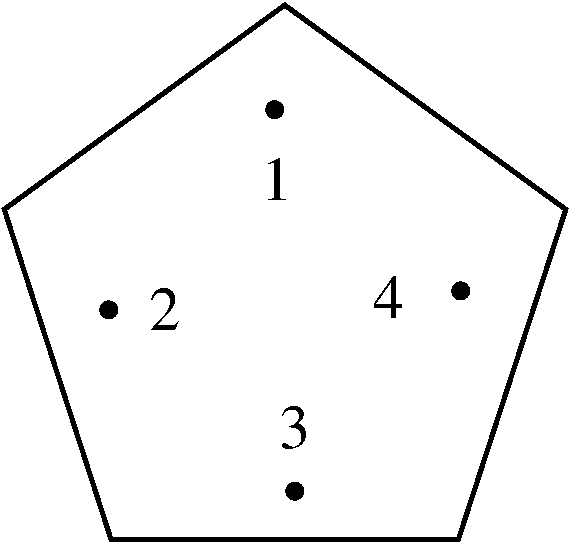
\includegraphics[width=4cm]{figures/pentagon_degree3.pdf}
    \hspace{1cm}
    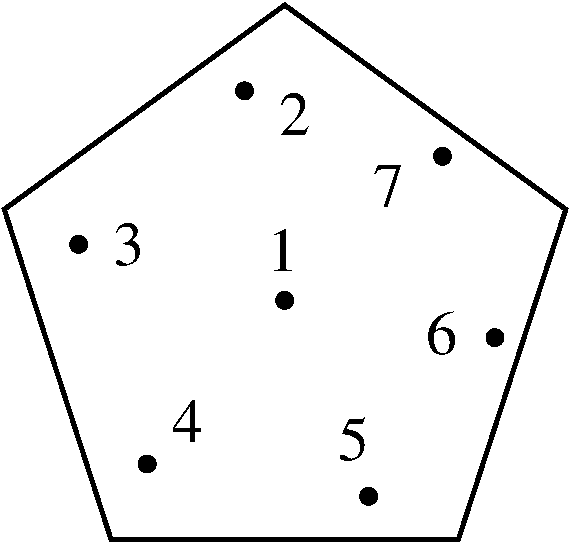
\includegraphics[width=4cm]{figures/pentagon_degree5.pdf}
    \caption{Locations of generalized, Gaussian, quadrature nodes for the $3^{\mathrm{rd}}$ (left) and $5^{\mathrm{th}}$ (right) degree integration methods presented in Table~\ref{tabQuadrature}.  Vertex 1 is located at the top of the pentagon, cf.\ Fig.~\ref{figRegPentagon}, while the coordinate origin is located at its centroid (node 1 in the right figure).}
    \label{figQuadrature}
\end{figure}

\subsection{Gauss Integration of Alveolar Sacs}

The quadrature rules that integrate a 2D tetrahedron in its natural co-ordinate system, where the apex is at the origin, and along its three axes: $0 \leq \xi \leq 1$, $0 \leq \eta \leq 1$ and $0 \leq \zeta \leq 1$.  These formul\ae\ integrate polynomials of $1^{\text{st}}$, $2^{\text{nd}}$ and $3^{\text{rd}}$ degrees, exactly, and can be found in most finite element textbooks.  

\begin{table}
    \centering
    \begin{tabular}{|c|rrrr|}
        \hline
        node & \centering $\xi$ co-ordinate & $\eta$ co-ordinate & 
        $\zeta$ co-ordinate & weight \\ \hline        
        & \multicolumn{4}{|c|}{Exact for Polynomials of Degree $1^{\phantom{|^|}}$} \\ 
        \hline
        1 & 1/4 & 1/4 & 1/4 & 1/6 \\ 
        \hline
        & \multicolumn{4}{|c|}{Exact for Polynomials of Degree $2^{\phantom{|^|}}$} \\ \hline
        1 & (5 - $\sqrt{5}$)/20 & (5 - $\sqrt{5}$)/20 & (5 - $\sqrt{5}$)/20 & 1/24\\
        2 & (5 - $\sqrt{5}$)/20 & (5 - $\sqrt{5}$)/20 & (5 + 3 $\sqrt{5}$)/20 & 1/24\\
        3 & (5 - $\sqrt{5}$)/20 & (5 + 3 $\sqrt{5}$)/20 & (5 - $\sqrt{5}$)/20 & 1/24\\ 
        4 & (5 + 3 $\sqrt{5}$)/20 & (5 - $\sqrt{5}$)/20 & (5 - $\sqrt{5}$)/20 & 1/24\\ 
        \hline
        & \multicolumn{4}{|c|}{Exact for Polynomials of Degree $3^{\phantom{|^|}}$} \\ \hline
        1 & 1/4 & 1/4 & 1/4 & -2/15 \\
        2 & 1/2 & 1/6 & 1/6 & 3/40\\
        3 & 1/6 & 1/2 & 1/6 & 3/40\\ 
        4 & 1/6 & 1/6 & 1/2 & 3/40 \\
        5 & 1/6 & 1/6 & 1/6 & 3/40 \\
        \hline
    \end{tabular}
    \caption{Generalized, Gaussian, quadrature weights and nodes for integrating over a tetrahedron in its natural co-ordinate system.  These weights sum to \textfrac{1}{6}, which is the volume of a tetrahedron measured in its natural co-ordinate system.}
    \label{tabQuadraturetetra}
\end{table} 
